  \chapter{20200707}
    \section{20200707}
        \subsection{chapter 3}
        本章, 主要介绍了刚体运动的运动学(kinematics)和动力学(dynamics); 其中主要定义了
        \begin{itemize}
          \item 位置和速度的关系(kinematics)
          \item 动力学表达式
          \item 12个状态量的表达式
        \end{itemize}
        首先介绍了\textcolor{red}{声明了MAV状态变量}, 12个, 
        其中, 和平移运动相关的三个位置变量(ned), 
        三个速度变量($u, v, \omega$, $i^{b}, j^{b}, k^{b}$), 
        三个角度(roll($F^{v2}$), pitch($F^{v1}$), yaw($F^{v}$)), 
        三个角速度($i^{b}, j^{b}, k^{b}$); 
        其次推导了\textcolor{red}{运动学, 即位置和速度的关系}, 
        我们需要将其从位置的导数即速度从体坐标系下转换到vehicle坐标系下进行计算.  
        因为位置是NED, 属于惯性坐标系下的值, 那么速度也是表示在惯性坐标系, 而惯性坐标系和vehicle坐标系三轴的指向是一样的, 唯一不一样的是二者的原点位置不同, 前者的原点位置是在地心, 后者是在MAV的质心, 且从体坐标系到vehicle存在确定的旋转矩阵, 故我们需要做这样的一个变换, 从而使其统一化;
        最后也推导了\textcolor{red}{动力学方程}, 针对牛顿第二定律的应用, 分别介绍了其在MAV的平移运动和旋转运动的动力学模型,
        \subsection{chapter 4}
        本章, 主要关注于力和力矩的梳理, 主要的来源是
        \begin{itemize}
          \item 重力(没有产生力矩)
          \item 空气动力($f_{a}, m_{a}$)
          \item 推力($f_{p}, m_{p}$)
          \item 大气的扰动, 即风速
        \end{itemize}
        关于重力, 推导出了其与欧拉角的数学关系式; 关于空气动力, 从纵向和横向两个方面进行了描述, 其中也介绍了无人机的控制平面, 包括 方向舵-副翼-升降舵无人机架构; 方向升降舵无人机架构; 升降翼舵无人机架构, 以及后二者和前者的转化关系式. 
    \clearpage
    \section{代码框架的梳理}
        结合框图来进行阐述
      
    \clearpage
    \section{simulation}
    \begin{figure}[htbp]
      \centering
      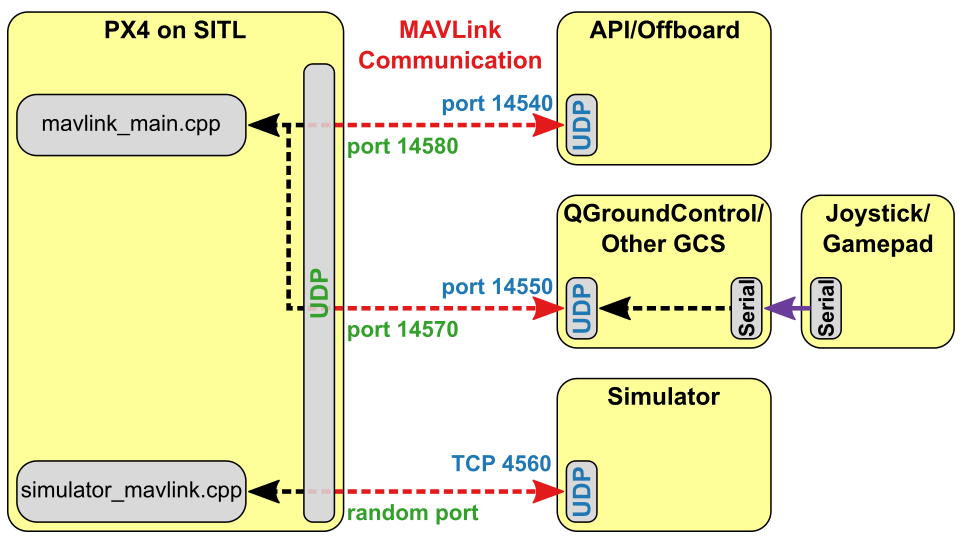
\includegraphics[width=0.8\textwidth]{pictures/chapter1/sitl.png}
      \caption{SITL}
    \end{figure}
    \begin{figure}[htbp]
      \centering
      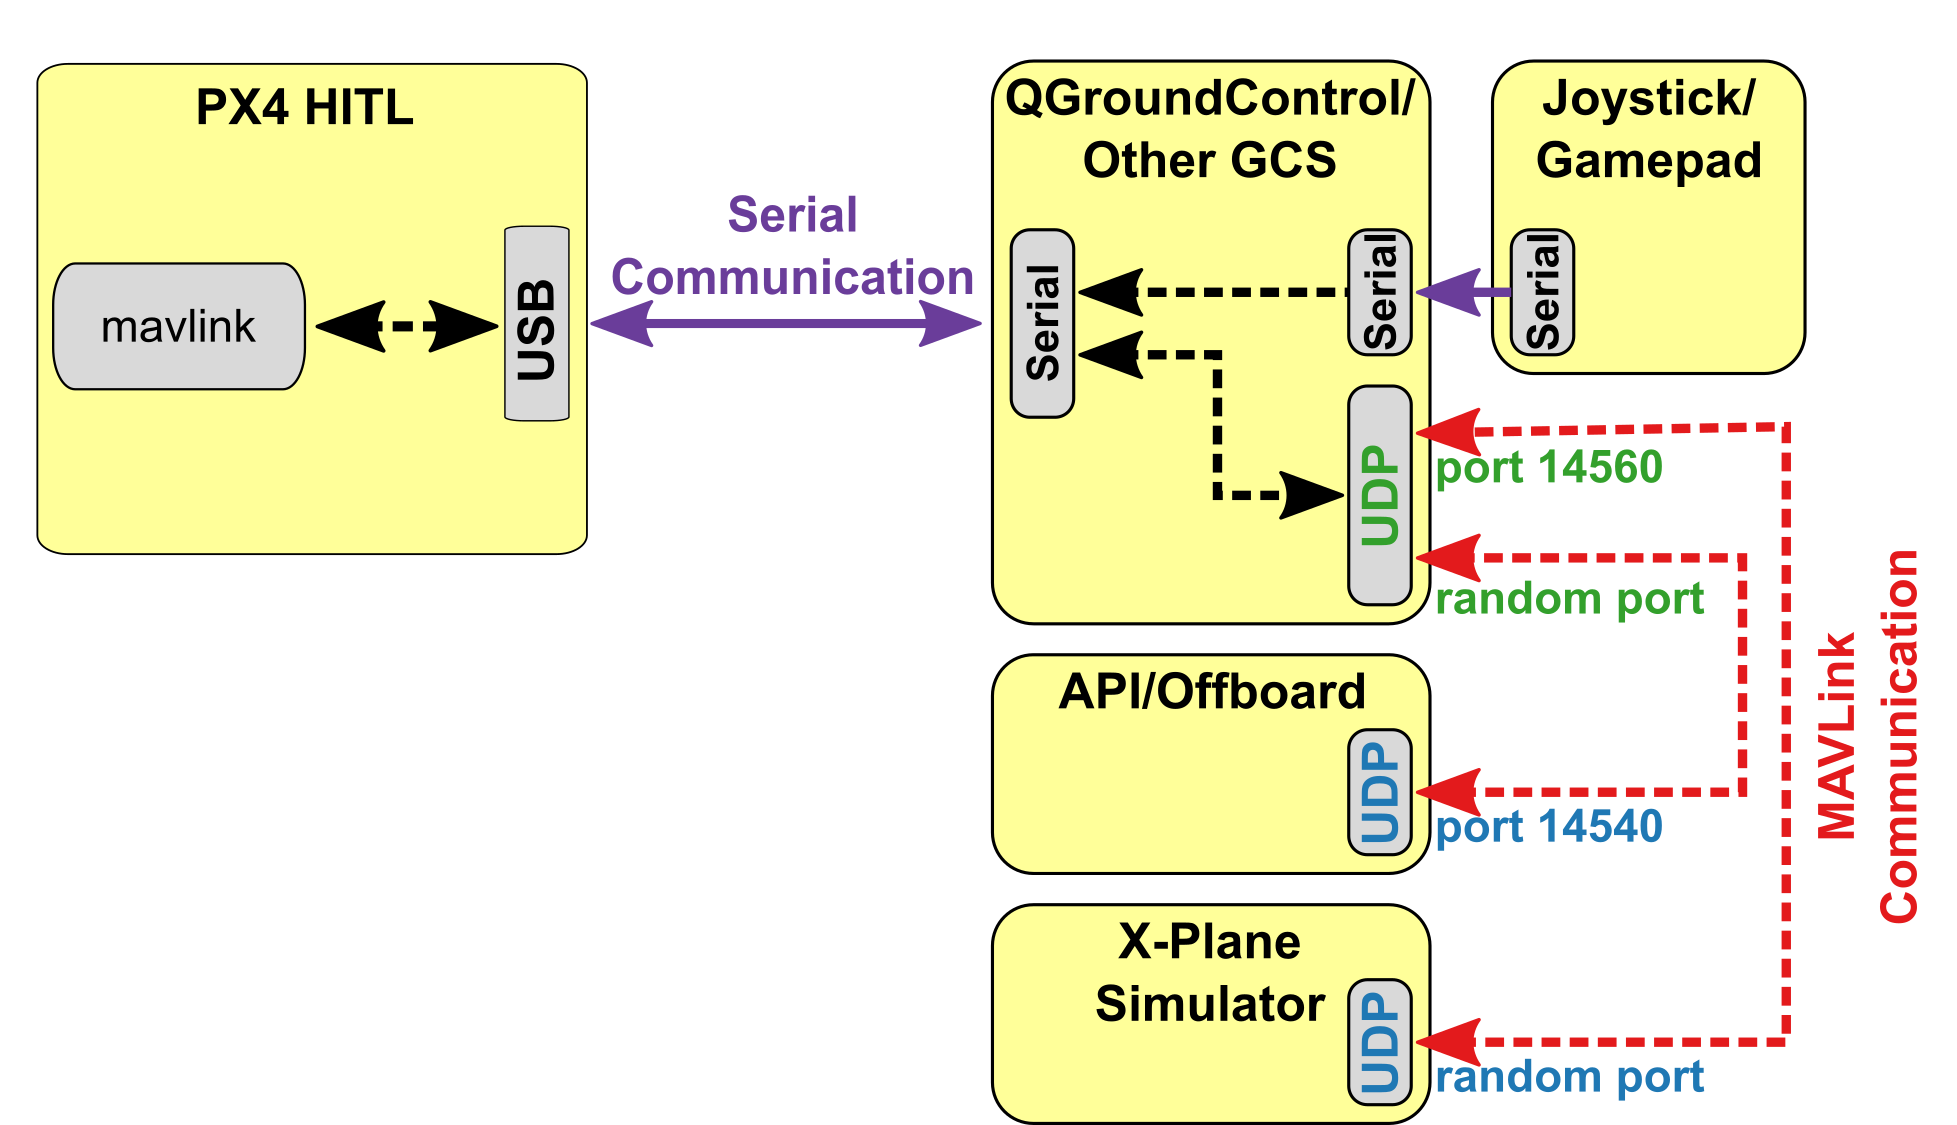
\includegraphics[width=0.8\textwidth]{pictures/chapter1/hitl.png}
      \caption{HITL-Xplane}
    \end{figure}
    \begin{figure}[htbp]
      \centering
      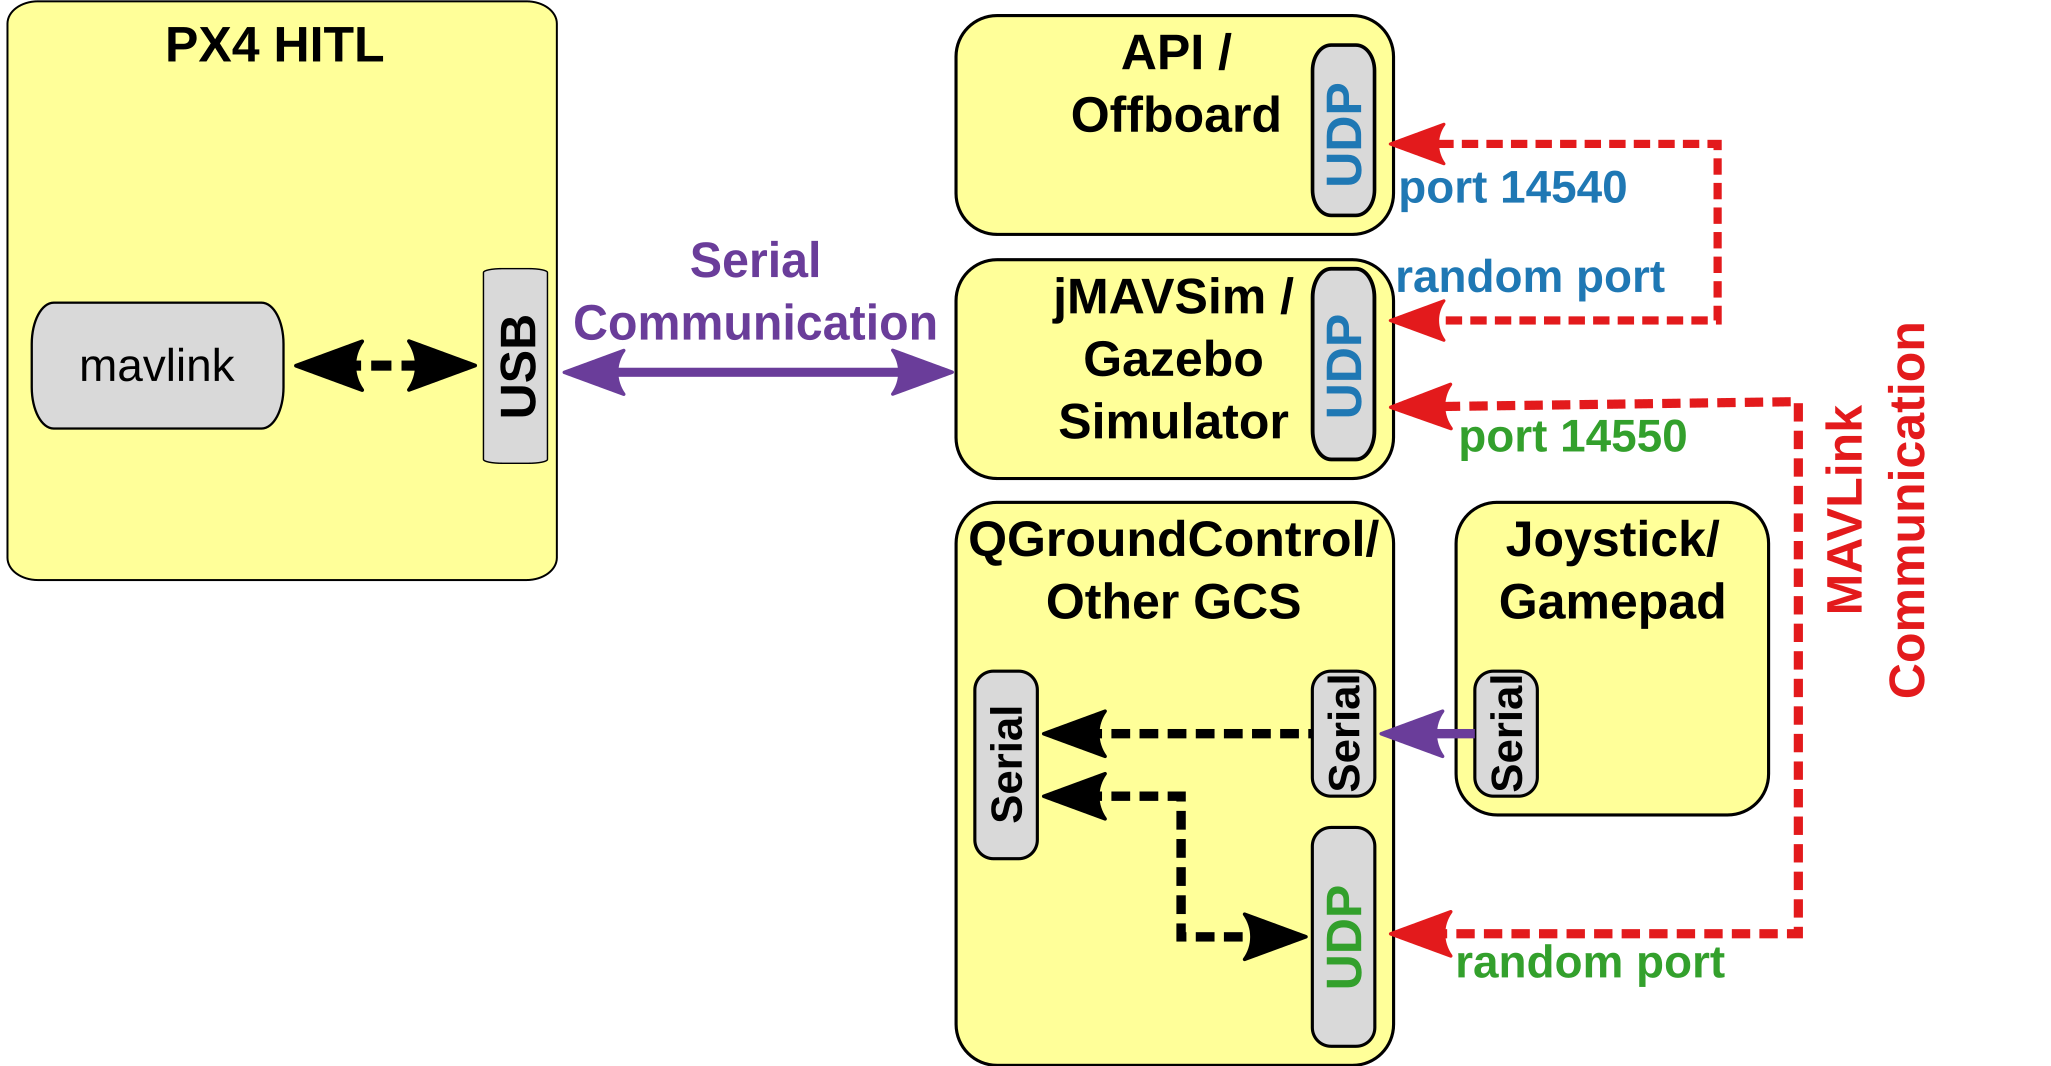
\includegraphics[width=0.8\textwidth]{pictures/chapter1/hitl2.png}
      \caption{HITL-Gazebo}
    \end{figure}
    \clearpage
    \section{计算机视觉}
        整理一下当前的任务流.
      计算机视觉, 是一门研究如何对数字图像或视频进行高层语义理解的交叉学科, 赋予了机器"看"的能力, 需要实现人的大脑中(主要是视觉皮层区)的视觉能力. \par
      图像处理, 用计算机对图像进行分析, 已达到所需结果的技术. 图像处理一般指的是数字图像处理, 图像处理的技术一般包括图像压缩, 增强和复原, 匹配, 描述和识别三个部分. 
      \par 图像处理就是各种的图像变换处理, 计算机视觉在图像处理之后再识别其内部的语义, 理解视频流中的内容. 
    \begin{figure}[htbp]
        \centering
        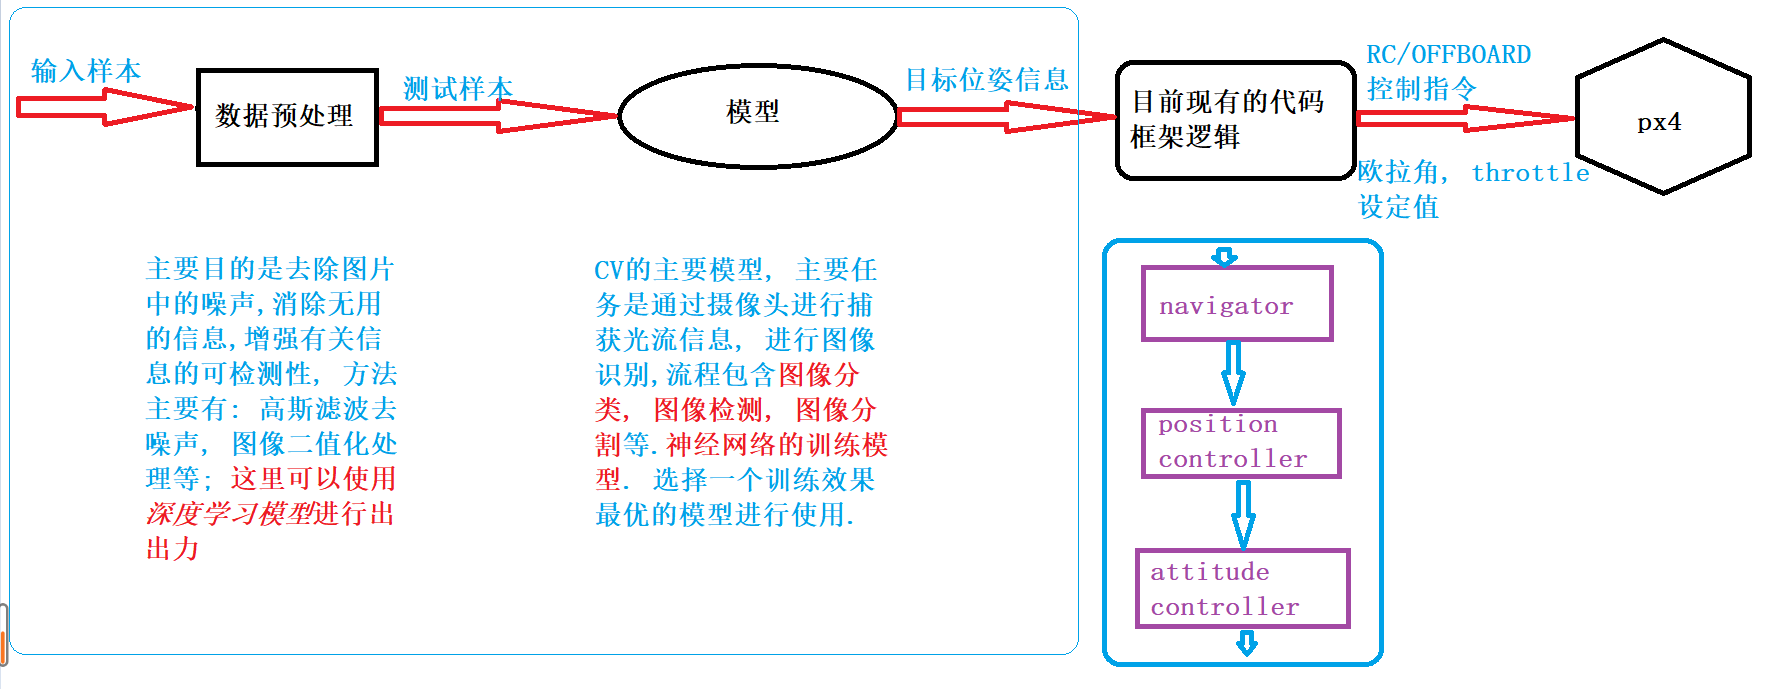
\includegraphics[width=0.8\textwidth]{pictures/chapter1/CV_Flow.png}
        \caption{CV数据流}
    \end{figure}  
    \clearpage
    \section{算法内部}
        有时间的话细说一下代码
% \end{document}
